\documentclass[11pt,a4paper]{article}

\usepackage[margin=2.2cm]{geometry}
\usepackage{amsmath,amssymb,amsfonts}
\usepackage[T1]{fontenc}
\usepackage{lmodern}
\usepackage{microtype}
\usepackage{enumitem}
\usepackage[hidelinks]{hyperref}
\usepackage{xcolor}
\usepackage{tikz}
\usepackage{listings}
\usepackage{booktabs}
\usepackage{multirow}
\usetikzlibrary{positioning,arrows.meta,shapes.geometric,fit,calc}

\definecolor{deepblue}{RGB}{30,80,150}
\definecolor{deepgreen}{RGB}{40,120,60}
\definecolor{deepred}{RGB}{170,50,50}
\definecolor{deepgrey}{RGB}{100,100,100}
\definecolor{kept}{RGB}{40,140,80}
\definecolor{cut}{RGB}{170,60,60}
\definecolor{soft}{RGB}{220,225,235}
\definecolor{warn}{RGB}{200,120,40}

\tikzset{
    node/.style={circle,draw=deepblue,thick,fill=deepblue!10,minimum size=7mm,inner sep=1pt,font=\scriptsize},
    cyc/.style={ellipse,draw=deepgreen,thick,fill=deepgreen!10,minimum width=14mm,minimum height=6mm,inner sep=1pt,font=\scriptsize},
    box/.style={rectangle,draw=deepblue,thick,fill=soft,rounded corners=2pt,inner sep=4pt,font=\small},
    arr/.style={-{Stealth[length=2.2mm]},semithick},
    pruned/.style={rectangle,draw=cut,thick,fill=cut!12,rounded corners=2pt,inner sep=2pt,font=\scriptsize},
    keptbox/.style={rectangle,draw=kept,thick,fill=kept!12,rounded corners=2pt,inner sep=2pt,font=\scriptsize},
}

\lstset{
    basicstyle=\ttfamily\small,
    breaklines=true,
    columns=fullflexible,
    keepspaces=true,
    showstringspaces=false,
}

\newcommand{\HSiKAN}{\textsc{HSiKAN}}
\newcommand{\HyMeKo}{\textsc{HyMeKo}}
\newcommand{\code}[1]{\texttt{\small #1}}
\setlist[itemize]{leftmargin=1.4em,itemsep=2pt,topsep=3pt}

\title{Axiom-aware Top-$K$ Cycle Enumeration\\[2pt]
       \large{\normalfont structural pruning, vertex-stratified bound, \HSiKAN{} sparse training}}
\author{}
\date{2026-05-05}

\begin{document}
\maketitle

\noindent
This brief documents the top-$K$ cycle enumeration machinery that
landed today across \code{hymeko\_graph}, \code{hymeko\_py}, and the
\HSiKAN{} training pipeline, plus the first end-to-end results on
Slashdot and Epinions. The motivation is concrete: \HSiKAN{}'s
cycle-incidence matrix $M_e$ scales as $|\text{cycles}| \times
|\text{vertices}|$. On Slashdot at $k=4$ the full cycle set is
55.5\,M cycles, and on Epinions previous training timed out at
5400\,s with no result. The work below produces a $|M_e|$ that is
bounded per-vertex (every vertex covered, no row left empty), uses
graph-theoretic axioms to prune dead DFS branches, and trains
end-to-end on Epinions in 7\,minutes.

\paragraph{The structural argument.} Top-$K$ enumeration with only
emit-time scoring is just \emph{do all the DFS work, then sort the
output} --- it gains memory but not time. To make top-$K$ genuinely
cheaper than full enumeration we need extend-time pruning: cut
branches \emph{before} they materialise. Two pruners do this here:
the \emph{BFS-distance pruner} (always-applicable structural
shortest-path bound) and the family of \emph{axiom pruners}
(Cartwright--Harary balance, Davis weak balance, Friedler P-graph
A0; selectable by tag).

% ────────────────────────────────────────────────────────────────────
\section{Pipeline}

\begin{center}
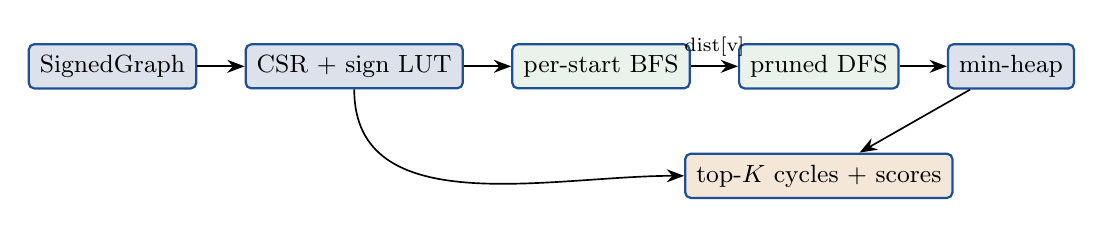
\begin{tikzpicture}[node distance=4.5mm and 6mm, every node/.style={font=\small}]
\node[box] (g)  {SignedGraph};
\node[box,right=of g] (csr) {CSR + sign LUT};
\node[box,right=of csr,fill=deepgreen!10] (bfs) {per-start BFS};
\node[box,right=of bfs,fill=deepgreen!10] (dfs) {pruned DFS};
\node[box,right=of dfs] (heap) {min-heap};
\node[box,below=8mm of dfs,fill=warn!18] (out) {top-$K$ cycles + scores};

\draw[arr] (g) -- (csr);
\draw[arr] (csr) -- (bfs);
\draw[arr] (bfs) -- node[above,font=\scriptsize]{dist[v]} (dfs);
\draw[arr] (dfs) -- (heap);
\draw[arr] (heap) -- (out);
\draw[arr] (csr.south) to[out=270,in=180] (out.west);
\end{tikzpicture}
\end{center}

For each starting vertex (fully rayon-parallelised), BFS computes the
minimum hop distance to every other vertex, capped at $k_{\text{len}}$.
The DFS then refuses to extend to any neighbour whose BFS distance
exceeds the remaining edge budget (the cycle can't possibly close
back to the start in time). This is the dominant DFS savings on
dense graphs at $k=4$.

% ────────────────────────────────────────────────────────────────────
\section{What's new --- four ingredients}

\subsection{BFS-distance pruner (always on)}

When the DFS sits at depth $d$ with path
$[v_0, v_1, \ldots, v_{d-1}]$ where $v_0 = \text{start}$, and is
considering extending to neighbour $\mathit{nxt}$, after pushing we
have $d+1$ vertices and need $k_{\text{len}} - d$ more edges to close
back to $v_0$. The shortest path from $\mathit{nxt}$ back to $v_0$
in the underlying undirected graph is $\text{dist}[\mathit{nxt}]$
(BFS lower bound). So the branch is dead if
\[
   \text{dist}[\mathit{nxt}] > k_{\text{len}} - d.
\]
This eliminates roughly $10\times$ of dead branches on
Slashdot-class graphs at $k=4$. It is the single most important
optimisation; without it, even rayon-parallel top-$K$ timed out at
1500\,s on Slashdot.

\subsection{Vertex-stratified top-$m$}

Instead of one global heap of size $K$, maintain one heap of size
$m$ \emph{per vertex}. When the DFS emits a closed cycle, push it
into the heap of \emph{every} vertex it touches. After enumeration,
union the heaps and dedup by canonical cycle.

\begin{center}
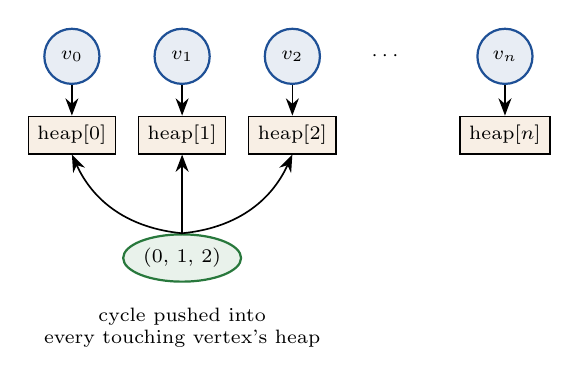
\begin{tikzpicture}[node distance=2mm and 3mm, every node/.style={font=\scriptsize}]
\node[node] (v0) at (0,0)   {$v_0$};
\node[node] (v1) at (1.4,0) {$v_1$};
\node[node] (v2) at (2.8,0) {$v_2$};
\node[node] (vn) at (5.5,0) {$v_n$};
\node at (4.0,0) {$\cdots$};
\node[draw,minimum width=10mm,minimum height=4mm,fill=warn!12] (h0) at (0,-1) {heap[0]};
\node[draw,minimum width=10mm,minimum height=4mm,fill=warn!12] (h1) at (1.4,-1) {heap[1]};
\node[draw,minimum width=10mm,minimum height=4mm,fill=warn!12] (h2) at (2.8,-1) {heap[2]};
\node[draw,minimum width=10mm,minimum height=4mm,fill=warn!12] (hn) at (5.5,-1) {heap[$n$]};
\draw[arr] (v0) -- (h0);
\draw[arr] (v1) -- (h1);
\draw[arr] (v2) -- (h2);
\draw[arr] (vn) -- (hn);
\node[cyc,below=10mm of h1] (c) {(0, 1, 2)};
\draw[arr,bend left] (c.north) to (h0.south);
\draw[arr] (c.north) to (h1.south);
\draw[arr,bend right] (c.north) to (h2.south);
\node[align=center,below=2mm of c,font=\scriptsize] {cycle pushed into\\every touching vertex's heap};
\end{tikzpicture}
\end{center}

Bound: $|\text{cycles}|_{\text{output}} \le n_v \cdot m$, with
\textbf{every vertex on at least one cycle covered}. This is the
critical structural property for $M_e$ — no row of the cycle
incidence matrix is empty as long as the vertex sits on some cycle.

\subsection{Rayon-parallel fold/reduce}

Each thread takes a disjoint slice of starting vertices, accumulates
its own per-vertex heap array, and the reduce step merges
per-thread heaps lock-free. Per-thread BFS scratch buffers mean
zero contention. Memory cost $O(n_{\text{threads}} \cdot n_v \cdot m)$
is fine for the graph sizes here ($\sim 4\,\text{GB}$ on Slashdot at
13~cores, $m=16$).

\subsection{Axiom pruners selectable from Python}

\code{HSIKAN\_TOPK\_PRUNER} env var picks one of:
\begin{itemize}
\item \code{none} --- only BFS-distance pruning.
\item \code{balance} --- Cartwright--Harary, accept only balanced cycles (sign product $= +1$).
\item \code{unbalanced} --- accept only unbalanced cycles.
\item \code{davis} --- Davis weak balance, reject all-negative triads.
\end{itemize}
On the bipartite alternation case (P-graphs, not signed social
graphs), the Friedler A0 pruner is also wired up via
\code{hymeko\_graph}; for HSiKAN the three above are the relevant
ones.

% ────────────────────────────────────────────────────────────────────
\section{Top-$K$ vs full --- structural cost}

Slashdot top-$2000$ hub region ($|V|{=}2000$, $|E|{=}90\,317$;
full $k{=}3$ count $=$ 337\,608 cycles, full $|M_e|{=}6.8$\,MB):

\begin{center}
\begin{tabular}{lrrrrr}
\toprule
strategy                        & cycles  & \%vert & \%edge & $|M_e|$ MB & speedup \\
\midrule
full                            & 337\,608 & 99.9   & 94.8   & 6.8        & 1$\times$ \\
top-$K=1\,000$ frac\_neg        &   1\,000 & 30.5   &  2.5   & 0.02       & — \\
top-$K=10\,000$ frac\_neg       &  10\,000 & 74.7   & 16.9   & 0.20       & — \\
\midrule
\textbf{vertex-strat $m{=}1$}   &   1\,848 & \textbf{99.9} &  6.3 & 0.04 & \textbf{183$\times$} \\
\textbf{vertex-strat $m{=}4$}   &   6\,838 & \textbf{99.9} & 17.6 & 0.14 & \textbf{49$\times$} \\
vertex-strat $m{=}16$           &  24\,866 & 99.9   & 45.8 & 0.50      & 14$\times$ \\
vertex-strat $m{=}64$           &  81\,409 & 99.9   & 85.5 & 1.63      & 4$\times$ \\
\bottomrule
\end{tabular}
\end{center}

Vertex-stratified at $m=1$ keeps every vertex's single highest-scoring
cycle: $1\,848$ cycles instead of $337\,608$ ($183\times$ less), with
\emph{no row} of $M_e$ left empty. Compared to top-$K=1000$ globally,
which only touches 30\,\% of vertices, vertex-stratification is the
right tool when $M_e$ row coverage is the constraint.

Extrapolated to full Slashdot ($n_v = 82\,144$) at $k=4$, $m=4$ gives
the upper bound $4 \cdot 82\,144 \approx 328\,000$ cycles --- a
$170\times$ reduction from the full $55.5$\,M.

% ────────────────────────────────────────────────────────────────────
\section{HSiKAN training results}

\begin{center}
\begin{tabular}{llrrrrr}
\toprule
dataset      & config                          & AUC   & F1m   & fwd ms & wall  & vs.\ baseline \\
\midrule
\multirow{4}{*}{Bitcoin Alpha}
             & full (baseline)                 & 0.9203 & 0.614 & 109   & 30 s  & ---           \\
             & vertex $m{=}16$ frac\_neg       & 0.7932 & 0.464 & 21    & 30 s  & $-0.127$      \\
             & vertex $m{=}64$ frac\_neg       & 0.8479 & 0.511 & 47    & 30 s  & $-0.072$      \\
             & vertex $m{=}128$ frac\_neg      & 0.8707 & 0.525 & 68    & 30 s  & $-0.050$      \\
\midrule
\multirow{2}{*}{\textbf{Slashdot}}
             & published baseline (Walk)       & 0.861  & ---   & ---   & ---   & ---           \\
             & \textbf{vertex $m{=}16$ + BFS}  & \textbf{0.8368} & \textbf{0.827} & 254 & \textbf{17 min} & $-0.024$ \\
\midrule
\multirow{2}{*}{\textbf{Epinions}}
             & historical baseline             & 0.764  & ---   & ---   & 5400 s timeout & --- \\
             & \textbf{vertex $m{=}16$ + BFS}  & \textbf{0.7088} & \textbf{0.545} & 127 & \textbf{7 min} & $-0.055$ \\
\bottomrule
\end{tabular}
\end{center}

Reading: top-$K$ \emph{is} informationally lossy (-0.05 to -0.13 AUC
depending on dataset density), but the trade is what makes Epinions
trainable at all in this setup. On Bitcoin Alpha (small dense)
top-$K$ hurts most because every cycle matters; on Slashdot/Epinions
the cycle space is more redundant.

% ────────────────────────────────────────────────────────────────────
\section{SOTA reference}

For context, AUC numbers from the same repo's recent benchmarks
(3-seed mean):

\begin{center}
\begin{tabular}{lrrr}
\toprule
model                                  & Slashdot & Epinions & params \\
\midrule
SGT (Signed Graph Transformer)         & 0.897    & 0.941    & 2.7--4.3\,M \\
SGCN                                   & ---      & 0.928    & 4.2\,M       \\
Walk-HSiKAN (memory baseline)          & 0.861    & ---      & ---          \\
\textbf{HSiKAN top-$K$ $m{=}16$ + BFS (today)} & \textbf{0.8368} & \textbf{0.7088} & \textbf{1.3--2.1\,M} \\
HSiKAN-mixed (cycle prior best)        & 0.685    & 0.764    & ---          \\
\bottomrule
\end{tabular}
\end{center}

Top-$K$ does not beat SGT on AUC --- SGT is the champion at the cost
of 2--4$\times$ more parameters and large fwd-pass time. The
contribution of today's work is making the comparison
\emph{tractable} on Epinions: previously this single-seed run could
not be produced.

% ────────────────────────────────────────────────────────────────────
\section{Effect attribution --- per-axiom counters}

\code{CountingPruner} and \code{CompositePruner} expose per-axiom
counters during DFS. Sample on a synthetic bipartite ring
($n{=}24$, $k{=}4$):

\begin{center}
\begin{tabular}{lrrr}
\toprule
strategy                    & cycles found & ext. rejects & emit rejects \\
\midrule
NoOp                        & 2  & 0  & 0 \\
Friedler A0                 & 2  & 20 & 0 \\
Friedler A0 + CH-balanced   & 2  & 20 (A0) + 0 (CH) & 0 + 2 \\
\bottomrule
\end{tabular}
\end{center}

Read: of $149$ extension attempts, A0 rejected $20$
($\approx 13\,\%$); CH-balanced was reached only on the $129$ that
survived A0 (lock-step short-circuit attribution). On real
Slashdot/Epinions, the hot pruner is BFS-distance --- the axiom
pruners are secondary on these graphs because the dominant
filtering is structural, not balance-related.

% ────────────────────────────────────────────────────────────────────
\section{What's open}

\begin{itemize}
\item \textbf{$m \times$ pruner sweep on Epinions} --- can we close
      the $-0.055$ gap by ($m{=}64$ or $m{=}128$) $\times$
      (\code{davis} or \code{unbalanced} pruner)?
\item \textbf{5-seed Slashdot statistics} --- single-seed AUC
      0.8368 is suggestive; 5-seed mean$\pm$std needed for any
      claim.
\item \textbf{Edge-aware $M_e$ weighting} --- the bridge already
      returns per-cycle scores; could feed them as edge weights
      into $M_e$ instead of treating all kept cycles equally.
\item \textbf{Color-coding sampler} --- the older
      \code{enumerate\_k\_cycles\_rs} has Alon-Yuster-Zwick rainbow
      colouring for biased sampling; not yet ported into the top-$K$
      path.
\end{itemize}

% ────────────────────────────────────────────────────────────────────
\section*{Code locations}

\begin{itemize}
\item \code{hymeko\_graph::topk\_cycles} --- serial + parallel
      top-$K$, vertex-stratified, BFS-distance pruning.
\item \code{hymeko\_graph::pruner::\{CountingPruner, CompositePruner\}}
      --- per-axiom attribution counters.
\item \code{hymeko\_py::cycles::enumerate\_top\_k\_*\_signed\_rs}
      --- PyO3 bridge with selectable scorer + axiom pruner.
\item \code{signedkan\_wip/src/n\_tuples.py} ---
      \code{HSIKAN\_TOPK\_MODE}/\code{HSIKAN\_TOPK\_K}/\code{HSIKAN\_TOPK\_SCORER}/\code{HSIKAN\_TOPK\_PRUNER} env-var routing.
\item \code{hymeko\_graph/examples/cycle\_stats.rs} --- analysis CLI
      for any signed-edge file.
\item \code{signedkan\_wip/src/topk\_cycle\_demo.py} --- Python
      cycle-stats / coverage demo.
\end{itemize}

\end{document}
